%!TEX program=lualatex
%!TEX options=-synctex=1 -interaction=nonstopmode -halt-on-error "%DOC%.tex"
\documentclass[11pt,pdfa,lastpage,minititle]{MishoNote}
\title{Remarks on Grading Policy and Conventions in Sho's Grading}
\author{Sho Iwamoto}
\hypersetup{
  pdflang={en-US},
  pdfauthortitle={Assistant Professor, National Sun Yat-sen University},
  pdfsubject={Notes on Sho's grading conventions},
  pdfcontactemail={iwamoto@g-mail.nsysu.edu.tw},
  pdfcontacturl={https://www2.nsysu.edu.tw/iwamoto/},
  pdfcaptionwriter={Sho Iwamoto},
  pdfcopyright={2023–2025 Sho Iwamoto},
  pdflicenseurl={https://www2.nsysu.edu.tw/iwamoto/},
}
\renewcommand\thesubsection{\arabic{subsection}.}
\begin{document}
\maketitle

This document outlines the grading policies for exams, quizzes, and assignments in Sho's lecture courses at National Sun Yat-sen University (NSYSU).
These policies apply only to Sho’s courses and not to those of other faculty members.

\subsection*{Overview}
The grading policy for Sho's courses at NSYSU should follow the \hrefFN{https://regs.nsysu.edu.tw/rule/rul_vie?rul=20190816111934}{university regulation}.
The method of calculating the final grade is stated in the syllabus (``Administrative Information'') of each course, which is designed with the following standards:
\begin{miniitemize}
  \item $\mathbfup{A+}$ for ``performance gone beyond Sho's expectation'',
  \item $\mathbfup{B-}$ for ``partial achievement of the lecture goals with some shortcomings'', and
  \item $\mathbfup{C-}$ for ``achievement of the minimum lecture goals but with major shortcomings''.
\end{miniitemize}
\OutputNote


\subsection*{Policy on the return of answer sheets}
In principle, Sho will not return your answer sheets.
\begin{itemize}
  \item First of all, Sho does not have ``the correct answer''.
  \item Sho wants students to be independent thinkers, not relying on the ``truth'' given by authority.
        They are asked to find the best solution by themselves, not to reach the same solution as Sho's.
\end{itemize}
Sho also thinks that returning answer sheets will have no effect to improve their learning, while it consumes significant time of Sho, which should be used for other educational activities.
\begin{itemize}
  \item Motivated students review it anyway, while unmotivated students do not review regardless of whether sheets are returned. Students usually focus only on their scores, not on the content.
  \item The primary purpose of exams is to evaluate achievement, not to provide feedback or promote further learning. If students need advice or feedback, they should ask before the exam.
  \item According to NSYSU regulations, faculty are not required to return answer sheets.
\end{itemize}
 However, the following cases are exceptions:
\begin{itemize}
  \item Mini tests. Sho designs them as an opportunity to provide feedback, rather than to evaluate achievement, so that they recognize shortcomings in their discussion and writing.
  \item Fall-semester lectures targeting first-year students. As they are not mature enough to behave as independent thinkers, Sho gives feedback for all mini tests and exams.
  \item During office hours. However, only if they rework over an exam or test and produce their own revised answers. They need to have in-person visits.
\end{itemize}

\subsection*{Mark Style}
Sho uses the following mark style to describe his opinion.

\begin{DownPara}
\begin{tabbing}
  \kern1.3em\=\kern1.3em\=\kern4.5em\=\kern7em\=\kill
  \JA{○}\>: Sho agrees with the answer.\\
  \JA{○}\kern-0.7em \raise0.3ex\hbox{\small\textsf s}\>: Sho agrees with it, but suspects mishandling of significant figures.\\
  \JA{×}\>: Sho thinks it is incorrect.\\
  \JA{△}\>: Sho thinks it worths partial mark (with a number $n$ $\to$ $n$\JA{折})\addnote{For $1\le n\le 9$, $\text{(full mark)}\times0.1n$. For $10\le n\le99$, $\text{(full mark)}\times0.01n$.}.\\[.5em]
  \textsf{ACCEPT}: Sho thinks it is a wrong answer but has decided to accept it as a correct answer.
\end{tabbing}
\end{DownPara}

\noindent The following symbols are used to describe Sho's feedback.
\begin{DownPara}
\begin{tabbing}
  \kern1.3em\=\kern1.3em\=\kern4.5em\=\kern7em\=\kill
  \fbox{\makebox[1.8em]{\textsf{UM}}}\>\>: unit missing\\
  \fbox{\makebox[1.8em]{\textsf{UE}}}\>\>: unit handling error\\
  \fbox{\makebox[1.8em]{\textsf{UD}}}\>\>: unit duplication\\
  \fbox{\makebox[1.8em]{\textsf{DM}}}\>\>: direction missing\\
  \fbox{\makebox[1.8em]{\textsf{DE}}}\>\>: direction error\\
  \fbox{\makebox[1.8em]{\textsf{Dir}}}\>\>: direction missing/error\\
  \fbox{\makebox[1.8em]{\textsf{VE}}}\>\>: vector handling error\\
  \fbox{\makebox[1.8em]{\textsf{Exp}}}\>\>: insufficient explanation\\
  \fbox{\makebox[1.8em]{\textsf{Calc}}}\>\>: calculation error\\[1em]

  underline ending with \JA{┘}\>\>\>\>: correct claim for partial mark\\
  underline ending with a number\>\>\>\>: correct claim for partial mark indicated by the number\\
  underline ending with \JA{×}\>\>\>\>: incorrect claim\\[1em]

  wavy underline\>\>\>: critical issue (usually it leads you to a wrong answer)\\
  purple marker\>\>\>: English issue (tolerated)\\
  yellow marker\>\>\>: minor issue (tolerated)\\
\end{tabbing}
\end{DownPara}

\noindent
(Sample: For a two-second free fall of a 5\,kg object, find the final kinetic energy and average speed.)
\begin{center}
  \fbox{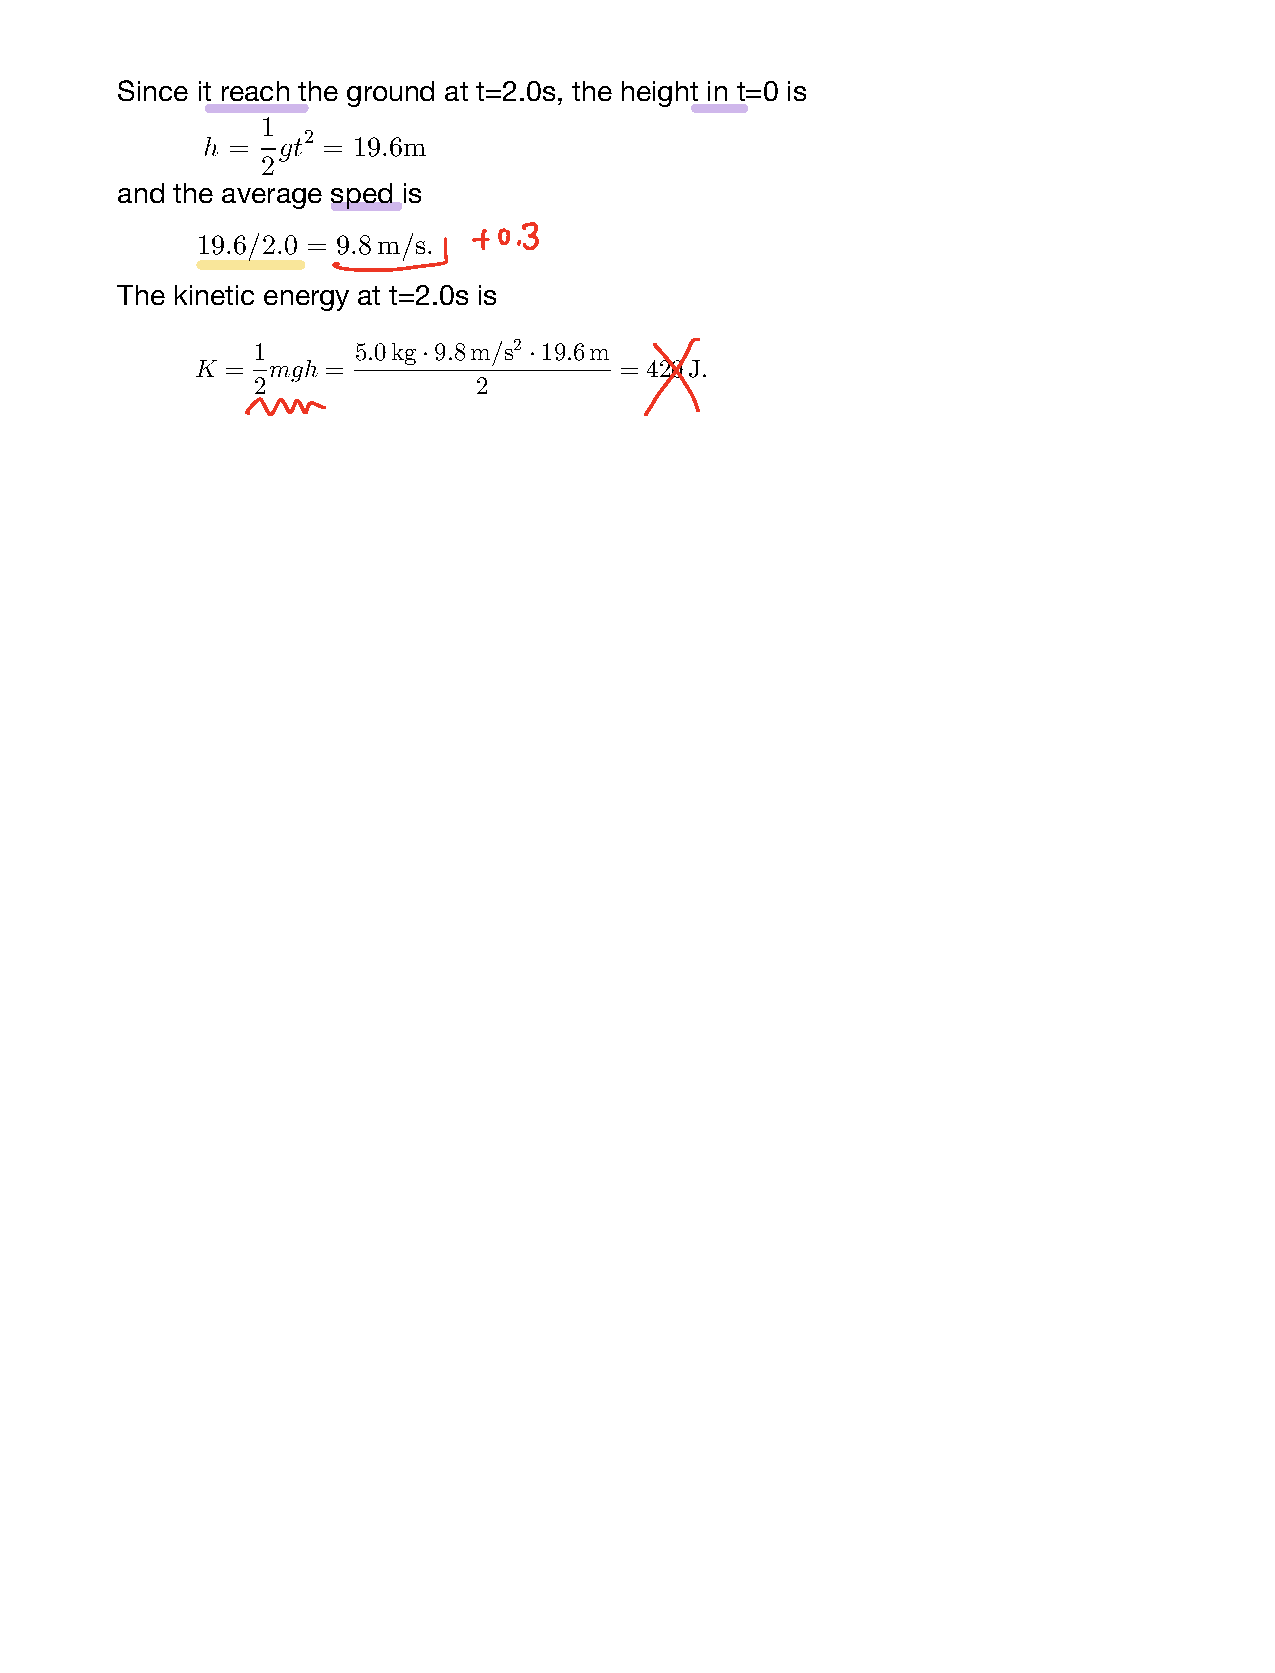
\includegraphics[width=0.6\textwidth]{grading_example.pdf}}
\end{center}

\OutputNote

\end{document}

